\documentclass{article}

\usepackage{lmodern}
\usepackage{hyperref}
\usepackage{amsmath}
\usepackage{amssymb}
\usepackage[T1]{fontenc}
\usepackage{fancyhdr}
\usepackage{color,graphicx}
\pagestyle{fancy}
\lhead{Anirudhan J. Rajagopalan --- ajr619}

\begin{document}

\title{Kernel Based Approaches for Change-Point Detection --- Report 1}
\date{February 18, 2016}
\author{Anirudhan J. Rajagopalan, ajr619}

\maketitle

\newpage
\section{Offline Detection}
\subsection{Univariate Detection}
Lets assume a time series of observations $x_{1}, x_{2}, \ldots, x_{n} $ of independent random variables with parameters $(\mu_{1}, \sigma_{1}^{2}), (\mu_{2}, \sigma_{2}^{2}), \ldots, (\mu_{n}, \sigma_{n}^{2}) $.
Also lets assume that each of the observation $ x_{i} $ is normally distributed with mean $ \mu $ and common variance $\sigma^{2} \forall i \in 1, 2, \ldots ,n $.
When there is no change in mean, the hypothesis of stability (null hypothesis) is defined as
\begin{align}
  H_{0} : \mu_{1} = \mu_{2} = \cdots =  \mu_{n} = \mu
\end{align}
Lets suppose that there is a change in the mean in the observations at an unknown point $ K $.  This can be define dy
\begin{align}
  H_{1} : \mu_{1} = \ldots \mu_{k} \ne \mu_{k+1} \ldots =  \mu_{n}
\end{align}
In our experiments we are going to assume that we know $\mu_{1}, \mu_{n} $ and $ \sigma $ are known beforehand (Refer $2.1.1$ of~\cite{birkhauser_pscpa}).

\subsubsection{Experiments}
Finding the likelihood directly using the likelihood function is not practical as it is not computationally tractable for even a small value of n (600 in our case).  So we follow the steps given in the reference\cite{birkhauser_pscpa} to find the change point.

The offline changepoint detection problem, gives a pretty accurate value for changepoint at k = 300.  The different plots are as displayed below.

\begin{figure}[ht!]
  \centering
  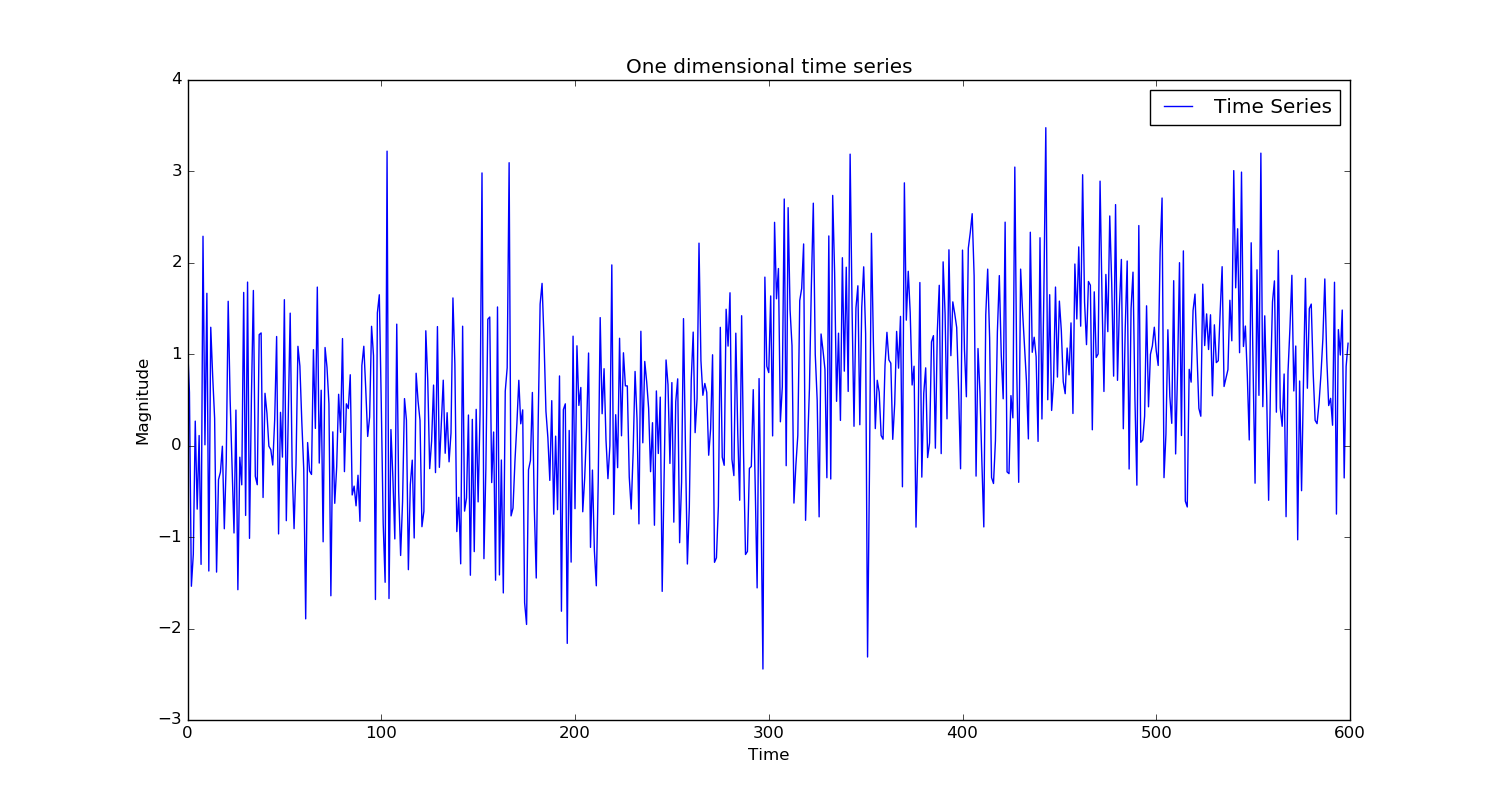
\includegraphics[width=1\textwidth]{images/1d_offline/ts}
  \caption{One dimensional time series.\label{fig:1d_ts}}
\end{figure}

\begin{figure}[ht!]
  \centering
  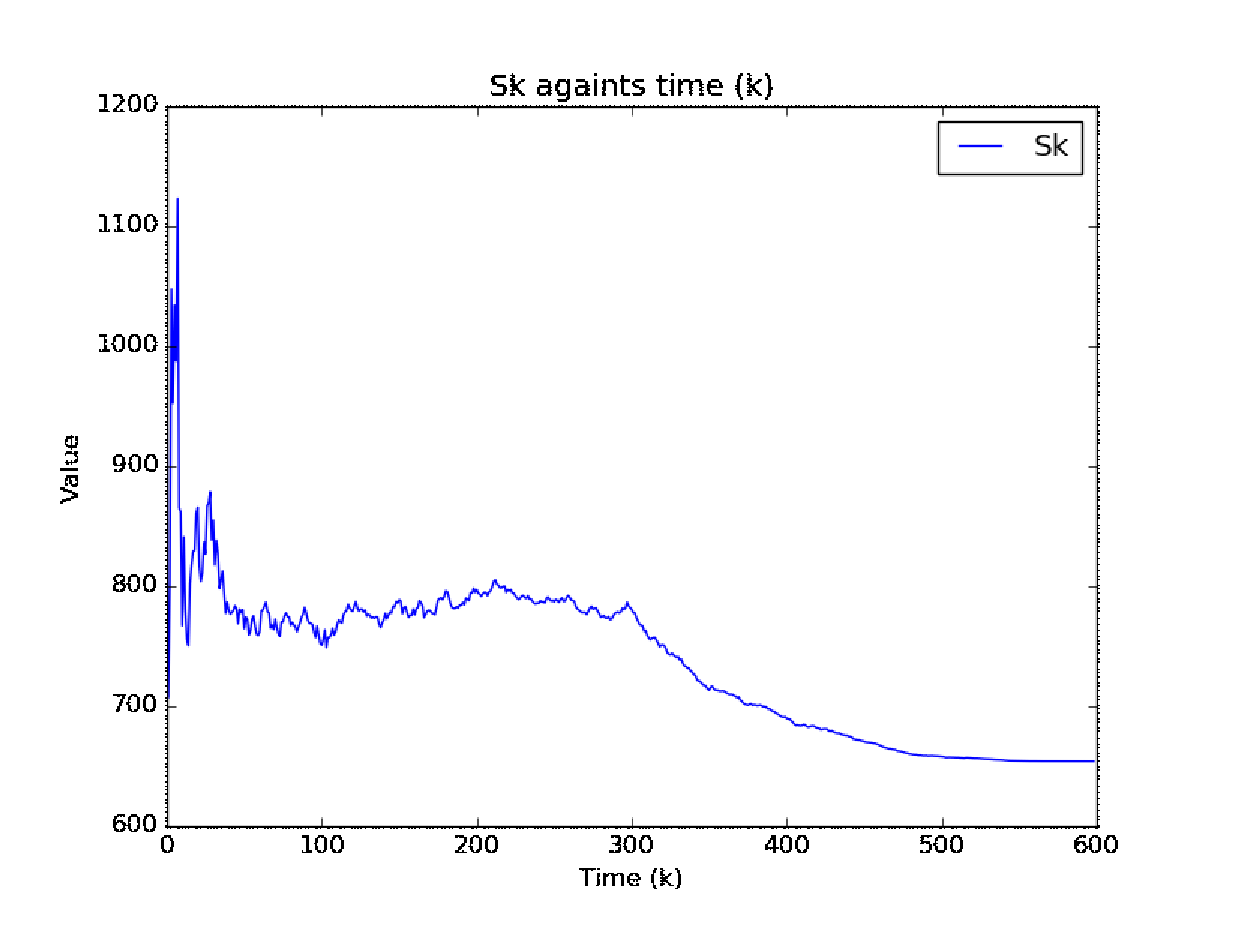
\includegraphics[width=0.75\textwidth]{images/1d_offline/sk}
  \caption{SK values for one dimensional offline detection problem.\label{fig:1d_sk}}
\end{figure}

\begin{figure}[ht!]
  \centering
  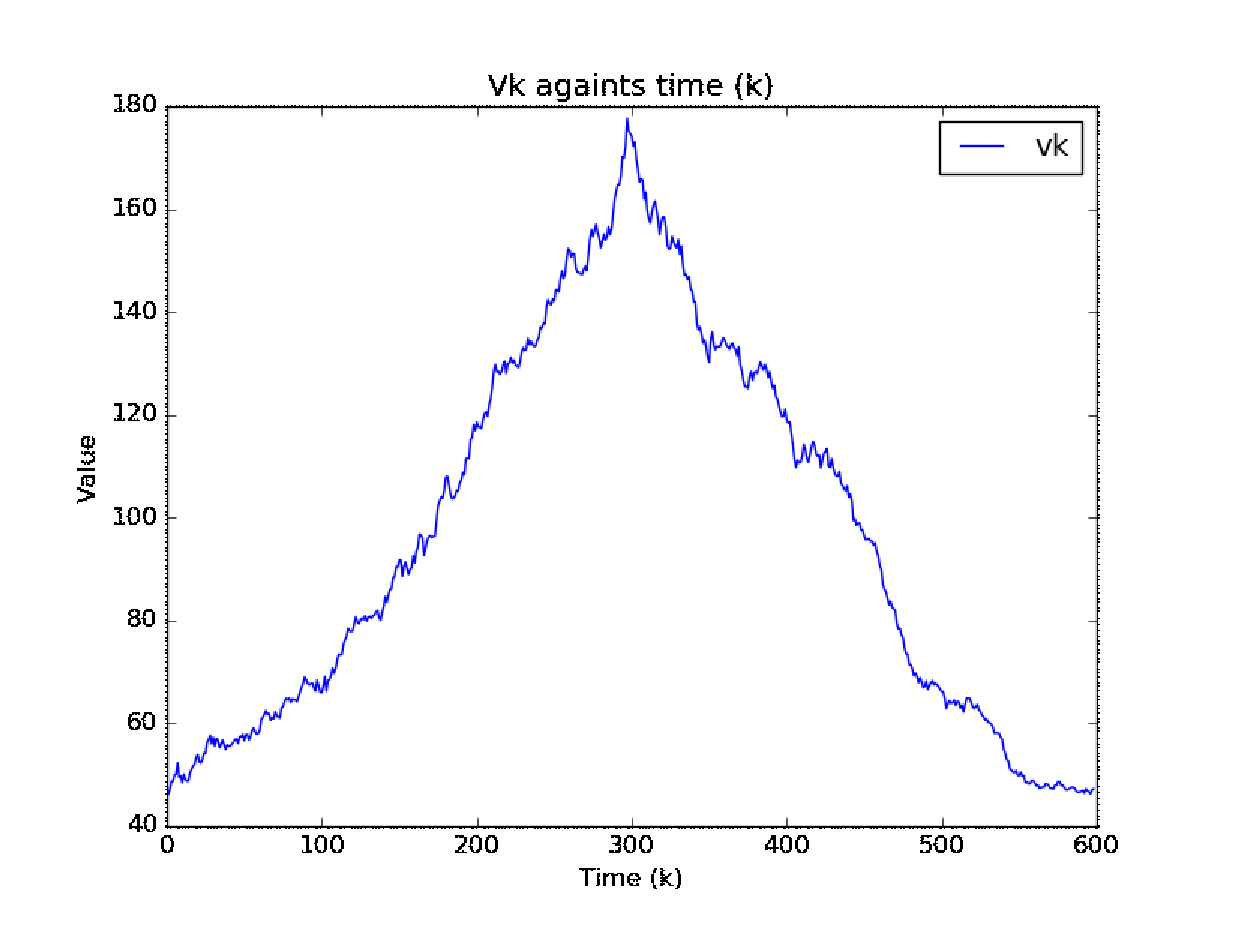
\includegraphics[width=0.75\textwidth]{images/1d_offline/vk}
  \caption{VK values for one dimensional offline detection problem.\label{fig:1d_vk}}
\end{figure}

\subsubsection{Questions \& Challenges}
\begin{enumerate}
  \item Finding how to derive sk, vk and $T^{2}$ test stastic for our own dataset when mean, and standard deviations are not known.
  \item Understanding what sk and vk represent.
\end{enumerate}

\subsection{Multi-variate Detection}
Multivariate model is similar to the above Univariate model except that each and every observation is m-dimensional.
Let $x_{1}, x_{2}, \ldots , x_{n}$ be a sequence of independent $m$-dimensional normal random vectors with parameters $(\mu_{1}, \Sigma_{1}), (\mu_{2}, \Sigma_{2}), \ldots, (\mu_{n}, \Sigma_{n})$, respectively.
Assume $\Sigma_{1} = \Sigma_{2} = \cdots = \Sigma_{n} = \Sigma $.
The null hypothesis is given by 
\begin{align}
H_{0} : \mu_{1} = \mu_{2} = \cdots = \mu_{n} = \mu (\mathrm{unknown})
\end{align}

If we assume that there is a change at point $k$ in the paramters governing the observation, then the hypothesis (alternate hypothesis) is given by

\begin{align}
H_{1} : \mu_{1} = \cdots = \mu_{k} \ne \mu_{k+1} = \mu_{n}
\end{align}
Where k represents the position of the single change point. (Refer 3.1 of~\cite{birkhauser_pscpa}).

This can be solved by following the steps described in section 3.1.1 of~\cite{birkhauser_pscpa}.  As in the case of univariate model, finding the likelihood directly is computationally intractable as $2\pi$ and $e$ has negative powers that can go pretty large and hence the likelihood will always become 1.

\subsection{Experiments}
We did Several experiments by varying the number of dimension and also the total number of samples.  So far, in all variations, we are able to identify the change point pretty accurately using the offline detection method described above.  The plots below are for dimension = 6 and number of samples = 600 with change point at 300.

\begin{figure}[ht!]
  \centering
  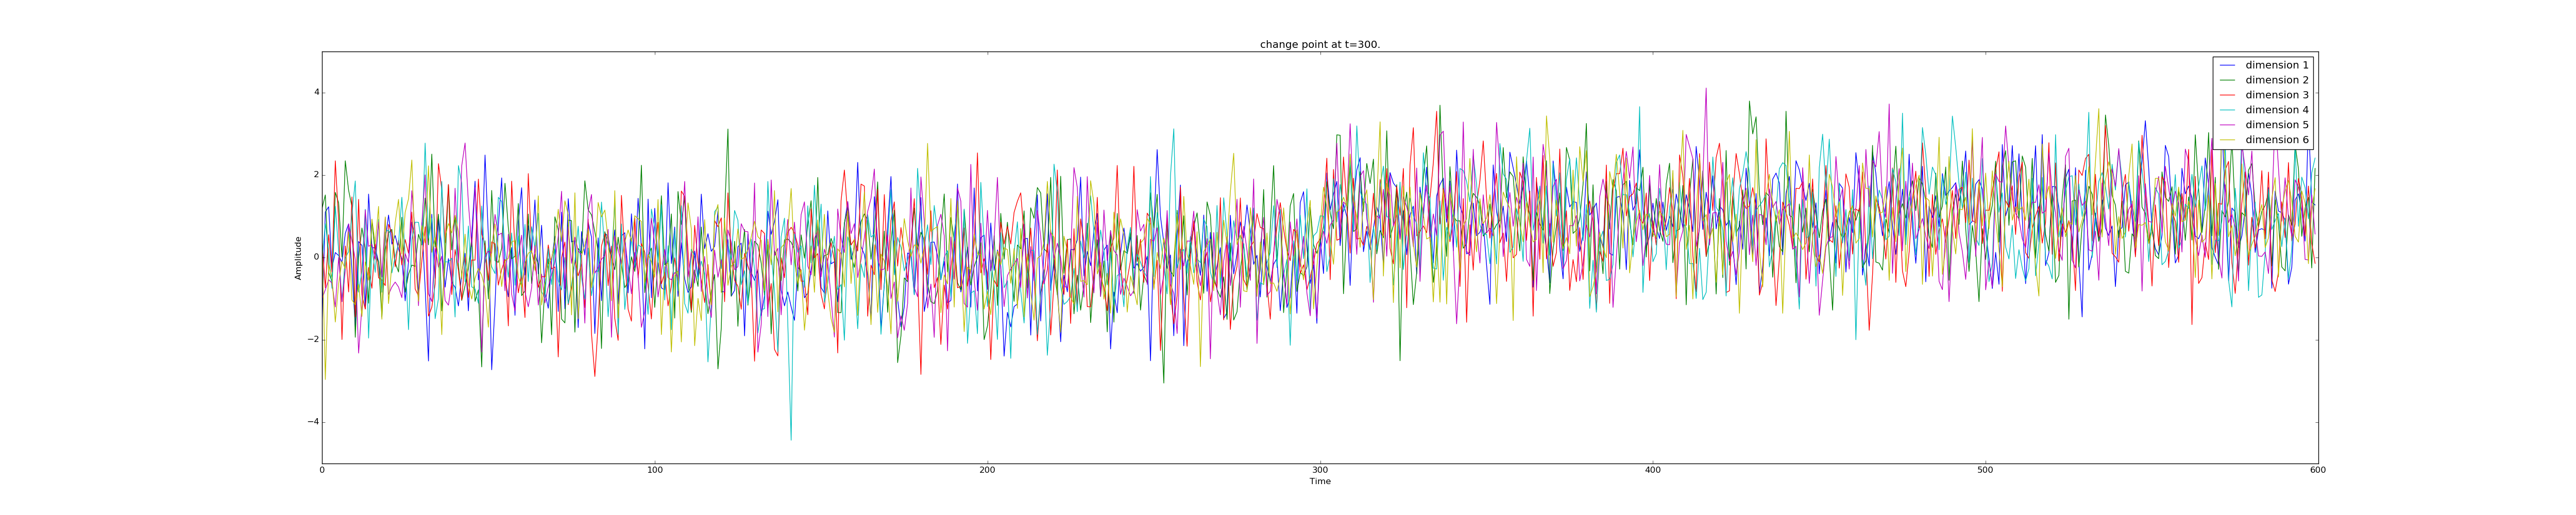
\includegraphics[width=1\textwidth]{images/rd_offline/ts}
  \caption{Multi dimensional time series.\label{fig:rd_ts}}
\end{figure}

\begin{figure}[ht!]
  \centering
  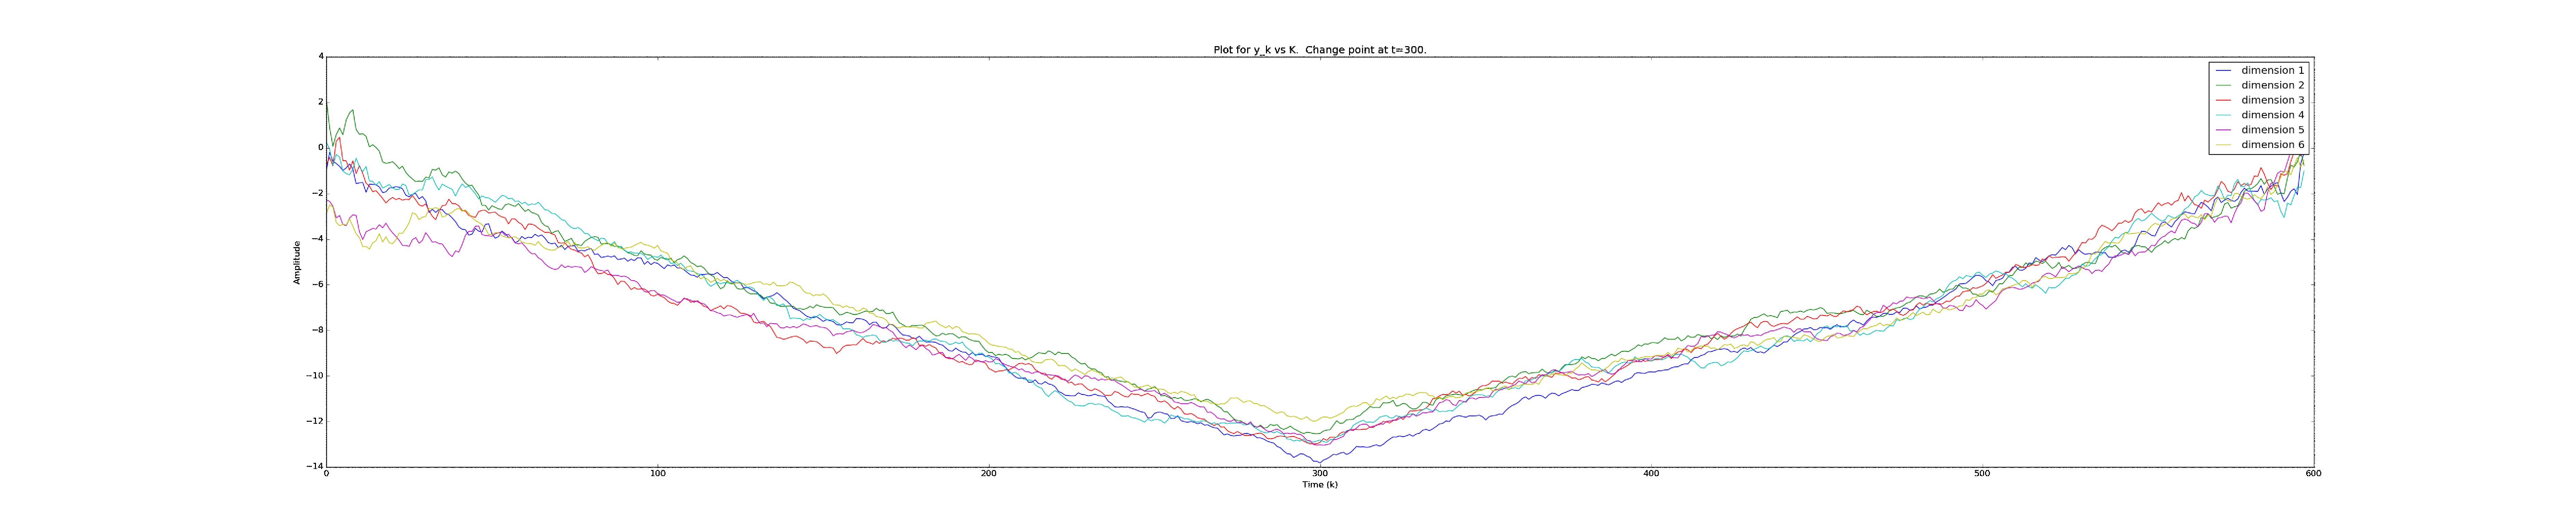
\includegraphics[width=1\textwidth]{images/rd_offline/y_k}
  \caption{Value of y\_k with respect to various k.\label{fig:rd_y_k}}
\end{figure}

\begin{figure}[ht!]
  \centering
  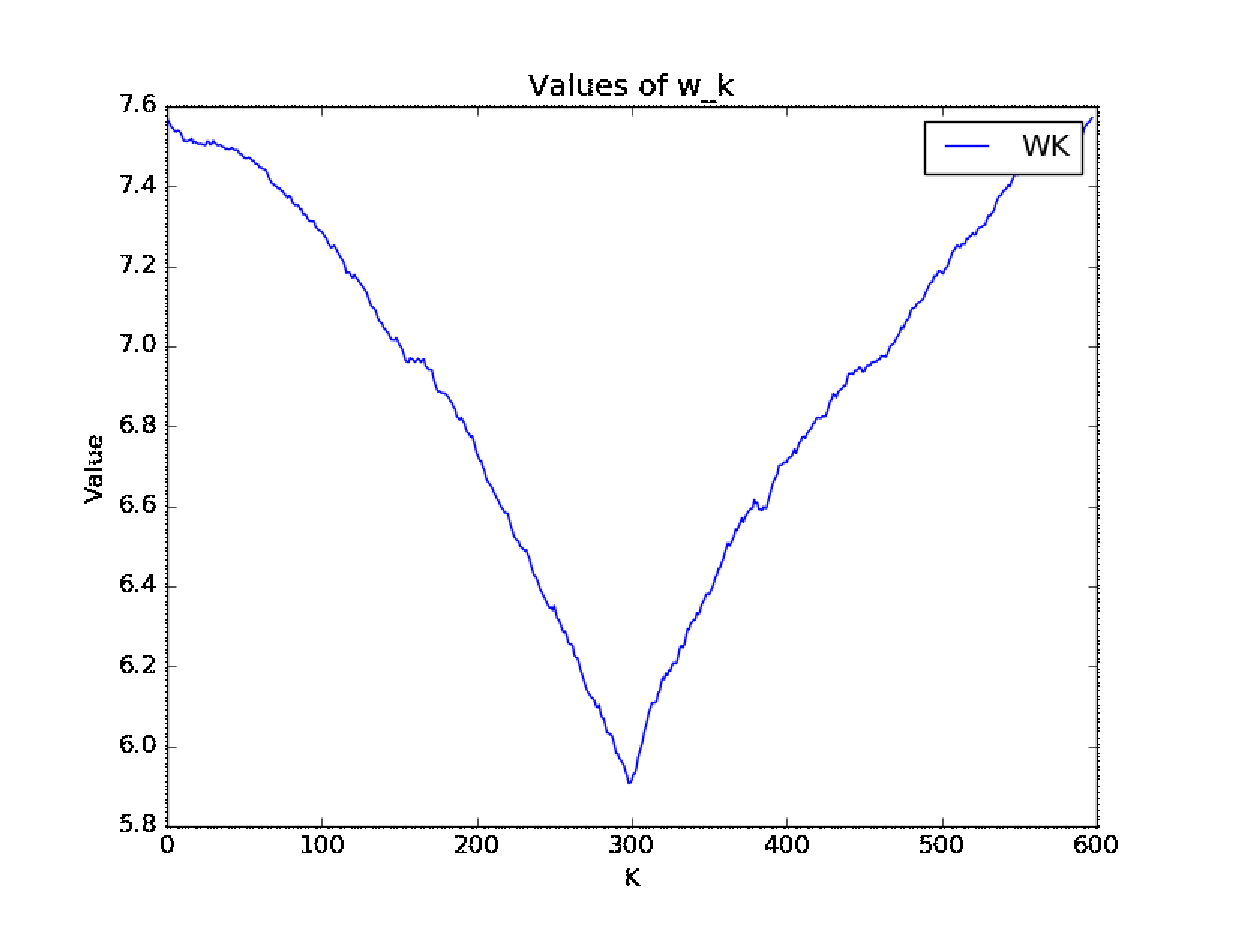
\includegraphics[width=0.75\textwidth]{images/rd_offline/w_k}
  \caption{Value of w\_k with respect to various k.\label{fig:rd_w_k}}
\end{figure}

\begin{figure}[ht!]
  \centering
  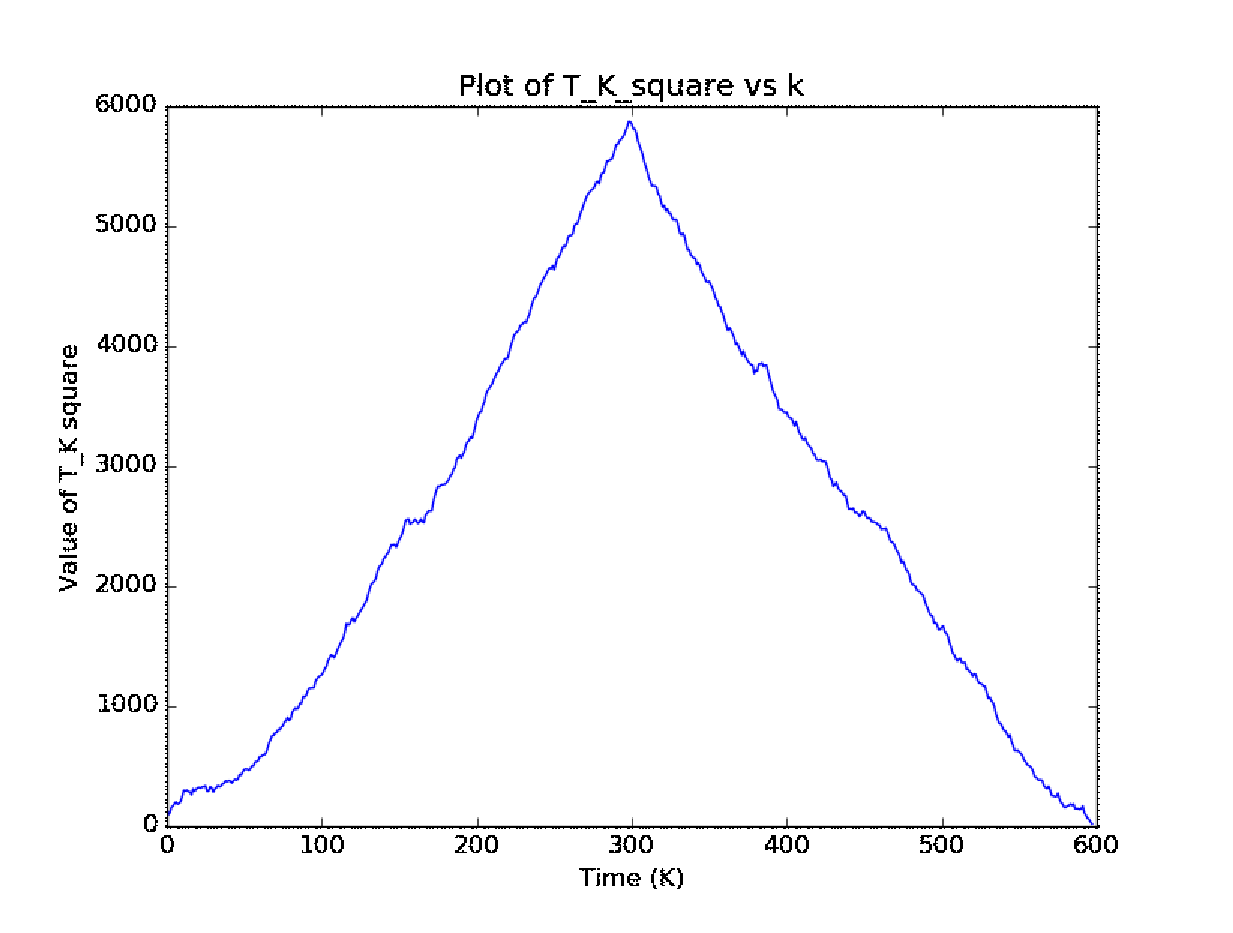
\includegraphics[width=0.75\textwidth]{images/rd_offline/tk_sq}
  \caption{Value of the test stastic $ T_{k}^{2} $ with respect to various k.\label{fig:rd_tk_sq}}
\end{figure}

\section{Online Detection}

\bibliographystyle{plain}
\bibliography{references}

\end{document}
